%%%%%%%%%%%%%%%%% KeOps presentation 22/01/2021 %%%%%%%%%%%%%%%%%%%%

\documentclass[14pt]{beamer}

%% theme
\usetheme{metropolis}

%% my style
\usepackage{mysettings}

%% custom commands


%% DOCUMENTS

\title[KeOps]{
\includegraphics[width=.5\linewidth]{./images/keops_logo.png}}
\subtitle{Seamless Kernel Operations on GPU without memory overflows}

\author{B. Charlier$^1$ \hfill J. Feydy$^2$ \hfill J. Glaun\`es$^3$ \hfill \textbf{G. Durif}$^1$ \hfill F.-D. Collin$^1$}
\date[]{\textit{January 22th 2021 -- State of the R}}
\institute[]{
$^1$IMAG - CNRS - Univ Montpellier, France, $^2$Imperial College, London, UK,\\ $^3$MAP5 - Univ Paris Descartes, France\\
~\\
\url{http://www.kernel-operations.io/}\\
\url{ghislain.durif@umontpellier.fr}
}

\begin{document}

\setlength{\parindent}{0pt}

%% TITLE PAGE
\begin{frame}
\maketitle

\end{frame}

%\footnotesize


\begin{frame}{Outline}
  \setbeamertemplate{section in toc}[sections numbered]
  \tableofcontents[hideallsubsections]
\end{frame}


%%%%%%%%%%%%%%%%%%%%%%%%%%%%%%%%%%%%%%%%%%%%%%%%%%%%%%%%%%%%%%%
\section{Introduction}
%%%%%%%%%%%%%%%%%%%%%%%%%%%%%%%%%%%%%%%%%%%%%%%%%%%%%%%%%%%%%%%


%%%%%%%%%%%%%%%%%%%%%%%%%%%%%%%%%%%%%%%
\begin{frame}{What is KeOps?}

\begin{center}
\url{http://www.kernel-operations.io/}\bigskip

KeOps = ``Kernel Operations''\bigskip

\begin{figure}
\centering

\includegraphics[width=.5\linewidth]{./images/rkeops_logo.png}
\end{figure}

RKeOps = \texttt{R} package interfacing KeOps library
\end{center}

\end{frame}

%%%%%%%%%%%%%%%%%%%%%%%%%%%%%%%%%%%%%%%
\begin{frame}{What KeOps can do?}

\only<1>{
\begin{center}
Compute \mybf{generic reductions} of very large arrays\bigskip\bigskip

{\small
\textit{e.g.} row-wise or column-wise matrix sum
\[
\sum_{i=1}^M a_{ij} \ \ \ \ \text{or}\ \ \ \ \sum_{j=1}^N a_{ij}
\]

\bigskip
(for some large matrix $\mb A = [a_{ij}] \in \RR^{M\times N}$)}
\end{center}
}

\only<2>{
\small
\[
\begin{array}{c}
\left[\begin{array}{cc>{\columncolor{mLightGreen}}ccc}
    \ \ \xx \ \  & \ \ \xx \ \  & \ \ \xx \ \ & \ \ \xx \ \ & \ \ \xx \ \ \\
    \ \ \xx \ \  & \ \ \xx \ \  & \ \ \xx \ \ & \ \ \xx \ \ & \ \ \xx \ \ \\
    \ \ \xx \ \ & \ \ \xx \ \ & a_{ij} & \ \ \xx \ \ & \ \ \xx \ \\\
    \ \ \xx \ \ & \ \ \xx \ \ & \ \ \xx \ \ & \ \ \xx \ \ & \ \ \xx \ \ \\
    \ \ \xx \ \ & \ \ \xx \ \ & \ \ \xx \ \ & \ \ \xx \ \ & \ \ \xx \ \ \\
  \end{array}\right]_{\myexample{M}\times\alert{N}}\\
  \downarrow \ \ \ \ \ \ \\
\left[\begin{array}{ccccc}
   \ \hdots \  & \hdots & \msum_{\myexample{i=1}}^{\myexample{M}} \myexample{a_{ij}} & \hdots & \ \hdots \ \\
  \end{array}\right]_{1\times\alert{N}}\\
\end{array}
\]
}

\only<3>{
\small
\[
\left[\begin{array}{ccccc}
    \ \ \xx \ \  & \ \ \xx \ \  & \ \ \xx \ \ & \ \ \xx \ \ & \ \ \xx \ \ \\
    \ \ \xx \ \  & \ \ \xx \ \  & \ \ \xx \ \ & \ \ \xx \ \ & \ \ \xx \ \ \\
   \rowcolor{mLightBrown}
    \ \ \xx \ \ & \ \ \xx \ \ & a_{ij} & \ \ \xx \ \ & \ \ \xx \ \\\
    \ \ \xx \ \ & \ \ \xx \ \ & \ \ \xx \ \ & \ \ \xx \ \ & \ \ \xx \ \ \\
    \ \ \xx \ \ & \ \ \xx \ \ & \ \ \xx \ \ & \ \ \xx \ \ & \ \ \xx \ \ \\
  \end{array}\right]_{\myexample{M}\times\alert{N}}\ \ \rw \ \ \left[\begin{array}{c}
    \vdots \\
    \vdots \\
    \msum_{\alert{j=1}}^{\alert{N}} \alert{a_{ij}} \\
    \vdots\\
    \vdots\\
  \end{array}\right]_{\myexample{M} \times 1}
\]
}

\only<4>{
Compute \mybf{kernel reduction}\smallskip

\[
\text{e.g.} \ \ \ \ \sum_{i=1}^M K(\mb x_i, \mb y_j)\ \ \ \ \text{or}\ \ \ \ \sum_{j=1}^N K(\mb x_i, \mb y_j)
\]

\medskip
and the associated \mybf{gradients}\medskip

{\small (for a kernel function $K$ and some data vectors $\mb x_i, \mb y_j\in\RR^D$)}\medskip

\begin{itemize}
\item[$\rw$] \textbf{Intuitively:} $\big[K(\mb x_i, \mb y_j)\big]\in \RR^{M\times N}$ = matrix whose elements are given by a \mybf{formula}
\end{itemize}
}

\only<5>{
\begin{itemize}
\setitsep{2em}
\item[$\rw$] manage \mybf{large dimensions}\medskip

\begin{itemize}
\setitsep{1em}
\item even larger than GPU memory
\item $M$ and $N$ $\approx 10^4, 10^5, 10^6$
\end{itemize}

\item[$\rw$] \mybf{fast computation on GPU without memory overflow}
\end{itemize}
}

\end{frame}


%%%%%%%%%%%%%%%%%%%%%%%%%%%%%%%%%%%%%%%
\begin{frame}{Kernels in Statistics and Learning}
\begin{itemize}
\setitsep{1.6em}
\item Kernel density estimation
\item Classification/Regression: SVM, K-NN, etc\ldots
\item Kernel embeddings to compare distributions
\item Interpolation and Kriging
\item Optimal Transport
\end{itemize}
\end{frame}


%%%%%%%%%%%%%%%%%%%%%%%%%%%%%%%%%%
\begin{frame}{Motivations}

\only<1>{
\begin{center}
GPU user-friendly computing?\bigskip\bigskip

Only a few solution for specific tasks in \texttt{R}\bigskip\bigskip

See \url{https://CRAN.R-project.org/view=HighPerformanceComputing} (section GPUs)
\end{center}
}

\only<2>{
Over the past 5 years: GPU computing development effort \mybf{oriented toward deep learning}\\
\medskip
\begin{itemize}
\item[$\rw$] e.g. PyTorch or TensorFlow provide {\bf GPU} implementation of common operations, together with {\bf automatic differentiation}.
\end{itemize}
}

\only<3>{
GPU computing can be used for \mybf{general purpose computations} and not only neural networks\\
\bigskip
\begin{itemize}
\item[$\rw$] Generic codes to use GPU computing require \textbf{low-level tools} (CUDA, OpenCL)
\end{itemize}
}

\only<4>{
\mybf{Needs:} provide an effortless tool for GPU computing\\

\bigskip

\textbf{Application:} statistics, machine learning and more\ldots
}
\end{frame}

%%%%%%%%%%%%%%%%%%%%%%%%%%%%%%%%%%%%%%%%%%%%%%%%%%%%%%%%%%%%%%%
\section{Kernel operations and reductions}
%%%%%%%%%%%%%%%%%%%%%%%%%%%%%%%%%%%%%%%%%%%%%%%%%%%%%%%%%%%%%%%

%%%%%%%%%%%%%%%%%%%%%%%%%%%%%%%%%%%%%%%%5
\begin{frame}{Kernel operator}

Considering some data vector $\mb x_i$ and $\mb y_j$ in $\RR^D$

\bigskip

\only<1>{
\medskip

(Intuitively)\smallskip

a \mybf{kernel} function = an application {\small $K: \RR^D \times \RR^D \to \RR$}
\[
(\mb x_i, \mb y_i) \mapsto K(\mb x_i, \mb y_i)
\]
corresponding to a \mybf{scalar product} between $\mb x_i$ and $\mb y_j$ in a different space than usual $\RR^D$
}

\only<2>{
\bigskip

(Very intuitively)

\begin{center}
a \mybf{kernel} function $\approx$ ``\textit{similarity measure}''\medskip

between $\mb x_i$ and $\mb y_j$\medskip

(different from Euclidean distance)
\end{center}
}

\btVFill

\end{frame}

%%%%%%%%%%%%%%%%%%%%%%%%%%%%%%%%%%%%%%%%5
\begin{frame}{Example}

Linear kernel
\[
K(\mb x_i, \mb y_j) = \big\langle \mb x_i \, , \, \mb y_j \big\rangle = \tr{\mb x_i}\,\mb y_j = \sum_{k=1}^D x_{ik}\,y_{jk}
\]
\medskip

Gaussian kernel
\[
K(\mb x_i, \mb y_j) = \exp\left(-\frac{1}{2\sigma^2}\Vertt \mb x_i - \mb y_j \Vertt_2^{\,2}\right)
\]

\end{frame}


%%%%%%%%%%%%%%%%%%%%%%%%%%%%%%%%%%%%%%%
\begin{frame}{Kernel reduction}

\bigskip
\begin{itemize}
\setitsep{1.5em}
\item \mybf{Row-wise or column-wise reduction} on the matrix $\mb K = \Big[K(\mb x_i, \mb y_j)\Big] \in \RR^{\myexample{M}\times\alert{N}}$
\item And more complex operations
\end{itemize}

\bigskip\bigskip

{\small
\textbf{Example:} \hfill \only<1>{$\sum_{\myexample{i=1}}^{\myexample{M}}\, K_1(\myexample{\mb x_i}, \mb y_j)\, K_2(\myexample{\mb u_i}, \mb v_j)\,\langle \myexample{\mbg\alpha_i}\,;\,\mbg\beta_j\rangle$}\only<2>{$\sum_{\alert{j=1}}^{\alert{N}}\, K_1(\mb x_i, \alert{\mb y_j})\, K_2(\mb u_i, \alert{\mb v_j})\,\langle \mbg\alpha_i\,;\,\alert{\mbg\beta_j}\rangle$} \hfill ~

\bigskip

for some kernel $K_1$ and $K_2$, and some $D$-vectors $(\mb x_i)_i, (\mb u_i)_i\\(\mbg\alpha_i)_i \in \RR^{\alert{M}\times D}$ and $(\mb y_j)_j, (\mb v_j)_j, (\mbg\beta_j)_j \in \RR^{\myexample{N}\times D}$}\bigskip

\end{frame}


%%%%%%%%%%%%%%%%%%%%%%%%%%%%%
%\begin{frame}{Generic reduction in KeOps}
%$1\leq i\leq N$ and $1 \leq j \leq M$ with $N,M \approx 10^4, 10^5, 10^6$\bigskip\bigskip
%
%
%\only<1>{
%\mybf{A generic case:}
%
%\[
%\small
%\left[ \sum_{\color{mLightBrown} j} F(\sigma_1,\cdots,\sigma_\ell,{\color{mLightGreen} X_i^1,\cdots,X^k_i},{\color{mLightBrown} Y^1_j,\cdots,Y^{m}_j}) \right]_{\myexample{i=1,\hdots,M}} \in \RR^{\myexample{M}}
%\]}
%
%\only<2>{
%\mybf{\ldots an even more generic case:}
%
%\[
%\small
%\left[ \Conv_{\color{mLightBrown} j} F(\sigma_1,\cdots,\sigma_\ell,{\color{mLightGreen} X_i^1,\cdots,X^k_i},{\color{mLightBrown} Y^1_j,\cdots,Y^{m}_j}) \right]_{\myexample{i=1,\hdots,M}} \in \RR^{\myexample{M}}
%\]
%
%where $\Conv$ can be any reduction (sum, max, min, etc.) over a dimension}
%
%\btVFill
%
%\end{frame}



%%%%%%%%%%%%%%%%%%%%%%%%%%%%
\begin{frame}{Why GPU computing?}

Matrix/kernel reduction = combination of generic matrix operations

\bigskip

\begin{center}
$\rw$ \mybf{GPU are good for matrix computations}
\end{center}

\end{frame}



%%%%%%%%%%%%%%%%%%%%%%%%%%%%%%%%%%%%%%%%%%%%%%%%%%%%%%%%%%%%%%%
\section{Computation on GPU}
%%%%%%%%%%%%%%%%%%%%%%%%%%%%%%%%%%%%%%%%%%%%%%%%%%%%%%%%%%%%%%%


%%%%%%%%%%%%%%%%%%%%%%%%%%%%
\begin{frame}{GPUs}

\textbf{PLUS}: thousands of computing units\medskip

$\rw$ fast with heavily parallelized computations\bigskip\bigskip

\textbf{MINUS}: relatively small memory\\
{\small(compared to the number of computing units)}\medskip

$\rw$ issue to process large data\bigskip

\end{frame}


%%%%%%%%%%%%%%%%%%%%%%%%%%%%
\begin{frame}{Challenge}

\begin{center}
Matrix $\mb K = \Big[K(\mb x_i, \mb y_j)\Big] \in \RR^{\myexample{M}\times\alert{N}}$ is very large\medskip

($M, N \approx 10^4, 10^5, 10^6$)
\end{center}

\begin{itemize}
\setitsep{2em}
\item[$\rw$] store it in memory? \mybf{NO!}
\item[$\rw$] how to iterate through rows/columns?
\end{itemize}

\end{frame}



%%%%%%%%%%%%%%%%%%%%%%%%%%%%%%%%%%%%%%%%%%%%%%%%%%%%%
\begin{frame}{Memory management on GPU}

\only<1>{
Data initially stored on the host (in RAM)\medskip
\begin{itemize}
\normalsize
\item[$\rw$] should be transfered to the device (GPU) for computations \mybf{(bottleneck)}
\end{itemize}\bigskip\bigskip

Different kinds of memory inside the GPU\medskip
\begin{itemize}
\normalsize
\item[$\rw$] local (smaller) vs shared (bigger) memory
\end{itemize}
}

\only<2>{
\mybf{Smart use of the shared memory}\bigskip
\begin{itemize}
\setitsep{1em}
\item[$\rw$] less transfer between device and host
\item[$\rw$] key to provide an efficient code in term of computational time
\end{itemize}

\begin{center}
\mybf{Tiling implementation}
\end{center}
\btVFill

\hyperlink{benchmark}{\beamerbutton{skip example}}
}

\end{frame}


%%%%%%%%%%%%%%%%%%%%%%%%%%%%%%%%%%%%%%%%%%%%%%%%%%%%%
\begin{frame}{Tiled implementation}

\only<1>{
Computations are divided into steps\bigskip\bigskip

Data are divided into blocks (called tiles)\bigskip\bigskip

Use of accumulators to combine intermediate results from each step on each block
}

\only<2>{
\mybf{Objective for massive parallel computing:}\medskip
\begin{itemize}
\setitsep{1.5em}
\item Shared memory stores data commonly used by all threads during a computation step\medskip

$\rw$ reduce transfers between host and GPU

\item Size of data only used by a single thread during a step is reduced (in local memory)\medskip

$\rw$ data locality

\end{itemize}
}

\end{frame}




%%%%%%%%%%%%%%%%%%%%%%%%
\begin{frame}{Example: matrix product}

%%
\begin{onlyenv}<1>
\begin{center}
$\mb A = [a_{ij}] \in \RR^{M\times N}$ and $\mb B = [b_{jk}] \in \RR^{N\times P}$\bigskip\bigskip

$\mb C = \mb A \,\mb B$\bigskip\bigskip

$\mb C = [c_{ik}] \in \RR^{M\times P}$ and $c_{ik} = \sum_j a_{ij}\,b_{jk} = \langle \mb a_{i \cdot}, \mb b_{\cdot k} \rangle$
\end{center}
\end{onlyenv}

%%
\begin{onlyenv}<2>
\footnotesize
\[
\begin{array}{c}
\left[\begin{array}{ccc}
\ \ \cdot \ \ & \ \ \cdot \ \  & \ \ \cdot \ \ \\
\hline
& \ \mb a_{i\cdot} & \\
 \hline
\ \ \cdot \ \ & \ \ \cdot \ \  & \ \ \cdot \ \ \\
\ \ \cdot \ \ & \ \ \cdot \ \  & \ \ \cdot \ \ \\
\end{array}\right]_{M \times N} \ \ \times \ \ \left[\begin{array}{c|c|c}
\ \ \cdot \ \ &   & \ \ \cdot \ \ \\
\ \ \cdot \ \ & \ \mb b_{\cdot k} \  & \ \ \cdot \ \ \\
\ \ \cdot \ \ & & \ \ \cdot \ \ \\
\end{array}\right]_{N \times P}\\
\\
= \ \ \left[\begin{array}{ccc}
\ \ \cdot \ \ & \ \ \cdot \ \  & \ \ \cdot \ \ \\
\ \ \cdot \ \ & \sum_j a_{ij}b_{jk} & \ \ \cdot \ \ \\
\ \ \cdot \ \ & \ \ \cdot \ \  & \ \ \cdot \ \ \\
\ \ \cdot \ \ & \ \ \cdot \ \  & \ \ \cdot \ \ \\
\end{array}\right]_{M \times P}
\end{array}
\]
\end{onlyenv}

%%
\begin{onlyenv}<3>
\small
\[
\begin{array}{ccc}
&& \left[\begin{array}{c|c|c}
\ \ \cdot \ \ \ \ \, &   & \, \ \ \ \ \cdot \ \ \\
\ \ \cdot \ \ \ \ \, & \ \ \mb b_{\cdot k} \ \ & \, \ \ \ \ \cdot \ \ \\
\ \ \cdot \ \ \ \ \, & & \, \ \ \ \ \cdot \ \ \\
\end{array}\right]_{N \times P}\\
\\
\left[\begin{array}{ccc}
\ \ \cdot \ \ & \ \ \cdot \ \  & \ \ \cdot \ \ \\
\hline
& \ \mb a_{i\cdot} & \\
 \hline
\ \ \cdot \ \ & \ \ \cdot \ \  & \ \ \cdot \ \ \\
\ \ \cdot \ \ & \ \ \cdot \ \  & \ \ \cdot \ \ \\
\end{array}\right]_{M \times N}
&& \left[\begin{array}{ccc}
\ \ \cdot \ \ & \ \ \cdot \ \  & \ \ \cdot \ \ \\
\ \ \cdot \ \ & \sum_j a_{ij}b_{jk} & \ \ \cdot \ \ \\
\ \ \cdot \ \ & \ \ \cdot \ \  & \ \ \cdot \ \ \\
\ \ \cdot \ \ & \ \ \cdot \ \  & \ \ \cdot \ \ \\
\end{array}\right]_{M \times P}
\end{array}
\]
\end{onlyenv}
\end{frame}

%%%%%%%%%%%%%%%%%%%%%%%%
\begin{frame}{Iterating through rows and columns}

%%
\begin{onlyenv}<1>
\small
\[
\begin{array}{cc}
& \left[\begin{array}{ccc}
\ \ \cl{\cdot} \ \ & \ \ \cdot \ \  & \ \ \cdot \ \ \\
\ \ \cl{\cdot} \ \ & \ \ \cdot \ \  & \ \ \cdot \ \ \\
\ \ \cl{\cdot} \ \ & \ \ \cdot \ \  & \ \ \cdot \ \ \\
\end{array}\right]\\
\\
\left[\begin{array}{ccc}
\ \ \cl{\cdot} \ \ & \ \ \cl{\cdot} \ \  & \ \ \cl{\cdot} \ \ \\
\ \ \cdot \ \ & \ \ \cdot \ \  & \ \ \cdot \ \ \\
\ \ \cdot \ \ & \ \ \cdot \ \  & \ \ \cdot \ \ \\
\ \ \cdot \ \ & \ \ \cdot \ \  & \ \ \cdot \ \ \\

\end{array}\right]
& \left[\begin{array}{ccc}
\ \ \cl{\cdot} \ \ & \ \ \cdot \ \  & \ \ \cdot \ \ \\
\ \ \cdot \ \ & \ \ \cdot \ \  & \ \ \cdot \ \ \\
\ \ \cdot \ \ & \ \ \cdot \ \  & \ \ \cdot \ \ \\
\ \ \cdot \ \ & \ \ \cdot \ \  & \ \ \cdot \ \ \\
\end{array}\right]
\end{array}
\]
\end{onlyenv}

%%
\begin{onlyenv}<2>
\small
\[
\begin{array}{cc}
& \left[\begin{array}{ccc}
\ \ \cdot \ \ & \ \ \cl{\cdot} \ \ & \ \ \cdot \ \ \\
\ \ \cdot \ \ & \ \ \cl{\cdot} \ \ & \ \ \cdot \ \ \\
\ \ \cdot \ \ & \ \ \cl{\cdot} \ \ & \ \ \cdot \ \ \\
\end{array}\right]\\
\\
\left[\begin{array}{ccc}
\ \ \cl{\cdot} \ \ & \ \ \cl{\cdot} \ \  & \ \ \cl{\cdot} \ \ \\
\ \ \cdot \ \ & \ \ \cdot \ \  & \ \ \cdot \ \ \\
\ \ \cdot \ \ & \ \ \cdot \ \  & \ \ \cdot \ \ \\
\ \ \cdot \ \ & \ \ \cdot \ \  & \ \ \cdot \ \ \\

\end{array}\right]
& \left[\begin{array}{ccc}
\ \ \cdot \ \ & \ \ \cl{\cdot} \ \  & \ \ \cdot \ \ \\
\ \ \cdot \ \ & \ \ \cdot \ \  & \ \ \cdot \ \ \\
\ \ \cdot \ \ & \ \ \cdot \ \  & \ \ \cdot \ \ \\
\ \ \cdot \ \ & \ \ \cdot \ \  & \ \ \cdot \ \ \\
\end{array}\right]
\end{array}
\]
\end{onlyenv}

%%
\begin{onlyenv}<3>
\small
\[
\begin{array}{cc}
& \left[\begin{array}{ccc}
\ \ \cdot \ \ & \ \ \cdot \ \ & \ \ \cl{\cdot} \ \ \\
\ \ \cdot \ \ & \ \ \cdot \ \ & \ \ \cl{\cdot} \ \ \\
\ \ \cdot \ \ & \ \ \cdot \ \ & \ \ \cl{\cdot} \ \ \\
\end{array}\right]\\
\\
\left[\begin{array}{ccc}
\ \ \cl{\cdot} \ \ & \ \ \cl{\cdot} \ \  & \ \ \cl{\cdot} \ \ \\
\ \ \cdot \ \ & \ \ \cdot \ \  & \ \ \cdot \ \ \\
\ \ \cdot \ \ & \ \ \cdot \ \  & \ \ \cdot \ \ \\
\ \ \cdot \ \ & \ \ \cdot \ \  & \ \ \cdot \ \ \\

\end{array}\right]
& \left[\begin{array}{ccc}
\ \ \cdot \ \ & \ \ \cdot \ \  & \ \ \cl{\cdot} \ \ \\
\ \ \cdot \ \ & \ \ \cdot \ \  & \ \ \cdot \ \ \\
\ \ \cdot \ \ & \ \ \cdot \ \  & \ \ \cdot \ \ \\
\ \ \cdot \ \ & \ \ \cdot \ \  & \ \ \cdot \ \ \\
\end{array}\right]
\end{array}
\]
\end{onlyenv}

%%
\begin{onlyenv}<4>
\small
\[
\begin{array}{cc}
& \left[\begin{array}{ccc}
\ \ \cl{\cdot} \ \ & \ \ \cdot \ \  & \ \ \cdot \ \ \\
\ \ \cl{\cdot} \ \ & \ \ \cdot \ \  & \ \ \cdot \ \ \\
\ \ \cl{\cdot} \ \ & \ \ \cdot \ \  & \ \ \cdot \ \ \\
\end{array}\right]\\
\\
\left[\begin{array}{ccc}
\ \ \cdot \ \ & \ \ \cdot \ \  & \ \ \cdot \ \ \\
\ \ \cl{\cdot} \ \ & \ \ \cl{\cdot} \ \  & \ \ \cl{\cdot} \ \ \\
\ \ \cdot \ \ & \ \ \cdot \ \  & \ \ \cdot \ \ \\
\ \ \cdot \ \ & \ \ \cdot \ \  & \ \ \cdot \ \ \\

\end{array}\right]
& \left[\begin{array}{ccc}
\ \ \cdot \ \ & \ \ \cdot \ \  & \ \ \cdot \ \ \\
\ \ \cl{\cdot} \ \ & \ \ \cdot \ \  & \ \ \cdot \ \ \\
\ \ \cdot \ \ & \ \ \cdot \ \  & \ \ \cdot \ \ \\
\ \ \cdot \ \ & \ \ \cdot \ \  & \ \ \cdot \ \ \\
\end{array}\right]
\end{array}
\]
\end{onlyenv}

%%
\begin{onlyenv}<5>
\small
\[
\begin{array}{cc}
& \left[\begin{array}{ccc}
\ \ \cdot \ \ & \ \ \cl{\cdot} \ \ & \ \ \cdot \ \ \\
\ \ \cdot \ \ & \ \ \cl{\cdot} \ \ & \ \ \cdot \ \ \\
\ \ \cdot \ \ & \ \ \cl{\cdot} \ \ & \ \ \cdot \ \ \\
\end{array}\right]\\
\\
\left[\begin{array}{ccc}
\ \ \cdot \ \ & \ \ \cdot \ \  & \ \ \cdot \ \ \\
\ \ \cl{\cdot} \ \ & \ \ \cl{\cdot} \ \  & \ \ \cl{\cdot} \ \ \\
\ \ \cdot \ \ & \ \ \cdot \ \  & \ \ \cdot \ \ \\
\ \ \cdot \ \ & \ \ \cdot \ \  & \ \ \cdot \ \ \\

\end{array}\right]
& \left[\begin{array}{ccc}
\ \ \cdot \ \ & \ \ \cdot \ \  & \ \ \cdot \ \ \\
\ \ \cdot \ \ & \ \ \cl{\cdot} \ \  & \ \ \cdot \ \ \\
\ \ \cdot \ \ & \ \ \cdot \ \  & \ \ \cdot \ \ \\
\ \ \cdot \ \ & \ \ \cdot \ \  & \ \ \cdot \ \ \\
\end{array}\right]
\end{array}
\]
\end{onlyenv}

%%
\begin{onlyenv}<6>
\small
\[
\begin{array}{cc}
& \left[\begin{array}{ccc}
\ \ \cdot \ \ & \ \ \cdot \ \ & \ \ \cl{\cdot} \ \ \\
\ \ \cdot \ \ & \ \ \cdot \ \ & \ \ \cl{\cdot} \ \ \\
\ \ \cdot \ \ & \ \ \cdot \ \ & \ \ \cl{\cdot} \ \ \\
\end{array}\right]\\
\\
\left[\begin{array}{ccc}
\ \ \cdot \ \ & \ \ \cdot \ \  & \ \ \cdot \ \ \\
\ \ \cl{\cdot} \ \ & \ \ \cl{\cdot} \ \  & \ \ \cl{\cdot} \ \ \\
\ \ \cdot \ \ & \ \ \cdot \ \  & \ \ \cdot \ \ \\
\ \ \cdot \ \ & \ \ \cdot \ \  & \ \ \cdot \ \ \\

\end{array}\right]
& \left[\begin{array}{ccc}
\ \ \cdot \ \ & \ \ \cdot \ \  & \ \ \cdot \ \ \\
\ \ \cdot \ \ & \ \ \cdot \ \  & \ \ \cl{\cdot} \ \ \\
\ \ \cdot \ \ & \ \ \cdot \ \  & \ \ \cdot \ \ \\
\ \ \cdot \ \ & \ \ \cdot \ \  & \ \ \cdot \ \ \\
\end{array}\right]
\end{array}
\]
\end{onlyenv}

\only<7>{
\begin{center}
and so on\ldots
\end{center}
}

\end{frame}

%%%%%%%%%%%%%%%%%%%%%%%%
\begin{frame}{Parallel matrix product}

\begin{onlyenv}<1-2>

Thread 1 and thread 2 \textbf{work in parallel}

\vspace{-0.3cm}

%%
\begin{onlyenv}<1>
\[
\scriptsize
\begin{array}{ccc}
&& \left[\begin{array}{ccc}
\ \ \cl{\cdot} \ \ & \ \ \cdot \ \  & \ \ \cdot \ \ \\
\ \ \cl{\cdot} \ \ & \ \ \cdot \ \  & \ \ \cdot \ \ \\
\ \ \cl{\cdot} \ \ & \ \ \cdot \ \  & \ \ \cdot \ \ \\
\end{array}\right]\\
\\
\begin{array}{r}
\text{thread 1 computes }T_1 \ \ \ \ \rw\\
\text{thread 2 computes }T_2 \ \ \ \ \rw\\
\\
\\
\end{array}
& \left[\begin{array}{ccc}
\bd & \bd & \bd \\
\uptri & \uptri & \uptri \\
\ \ \cdot \ \ & \ \ \cdot \ \  & \ \ \cdot \ \ \\
\ \ \cdot \ \ & \ \ \cdot \ \  & \ \ \cdot \ \ \\
\end{array}\right]
& \left[\begin{array}{ccc}
\ T_1 \ & \ \ \cdot \ \  & \ \ \cdot \ \ \\
\ T_2 \ & \ \ \cdot \ \  & \ \ \cdot \ \ \\
\ \ \cdot \ \ & \ \ \cdot \ \  & \ \ \cdot \ \ \\
\ \ \cdot \ \ & \ \ \cdot \ \  & \ \ \cdot \ \ \\
\end{array}\right]
\end{array}
\]
\end{onlyenv}

%%
\begin{onlyenv}<2>
\[
\scriptsize
\begin{array}{ccc}
&& \left[\begin{array}{ccc}
\ \ \cl{\cdot} \ \ & \ \ \cdot \ \  & \ \ \cdot \ \ \\
\ \ \cl{\cdot} \ \ & \ \ \cdot \ \  & \ \ \cdot \ \ \\
\ \ \cl{\cdot} \ \ & \ \ \cdot \ \  & \ \ \cdot \ \ \\
\end{array}\right]\\
\\
\begin{array}{r}
\\
\\
\text{thread 1 computes }T_1 \ \ \ \ \rw\\
\text{thread 2 computes }T_2 \ \ \ \ \rw\\
\end{array}
& \left[\begin{array}{ccc}
\ \ \cdot \ \ & \ \ \cdot \ \  & \ \ \cdot \ \ \\
\ \ \cdot \ \ & \ \ \cdot \ \  & \ \ \cdot \ \ \\
\bd & \bd & \bd \\
\uptri & \uptri & \uptri \\
\end{array}\right]
& \left[\begin{array}{ccc}
\ \ \cdot \ \ & \ \ \cdot \ \  & \ \ \cdot \ \ \\
\ \ \cdot \ \ & \ \ \cdot \ \  & \ \ \cdot \ \ \\
\ T_1 \ & \ \ \cdot \ \  & \ \ \cdot \ \ \\
\ T_2 \ & \ \ \cdot \ \  & \ \ \cdot \ \ \\
\end{array}\right]
\end{array}
\]
\end{onlyenv}

\vspace{0.3cm}

\begin{columns}
\begin{column}{0.5\textwidth}
\footnotesize
$\scriptsize\begin{array}{c}\cl{\ \ \ }\end{array}$ = shared data between threads
\end{column}
\begin{column}{0.5\textwidth}
\footnotesize
$\bd$ = data only used by thread 1\\
$\uptri$ = data only used by thread 2
\end{column}
\end{columns}
\end{onlyenv}

\begin{onlyenv}<3>

\textbf{Potential issues} if dimension $N$ is large {\small (nb. of columns in matrix $\mb A$)}

\begin{itemize}
\setitsep{1em}
\item[$\rw$] parallel threads are asynchronous and have to wait each other before updating shared memory (= using next column of matrix $\mb B$)
\item[$\rw$] rows of $\mb A$ are too large to fit into local memory used by each thread, hence numerous memory transfer
\end{itemize}

\end{onlyenv}
\end{frame}



%%%%%%%%%%%%%%%%%%%%%%%%
\begin{frame}{Tiled implementation}

\begin{onlyenv}<1-3>

Thread 1 and thread 2 \textbf{work in parallel}

\vspace{-0.3cm}

%%
\begin{onlyenv}<1>
\[
\scriptsize
\begin{array}{ccc}
&& \left[\begin{array}{ccc}
\ \ \cl{\cdot} \ \ & \ \ \cl{\cdot} \ \  & \ \ \cl{\cdot} \ \ \\
\ \ \cdot \ \ & \ \ \cdot \ \  & \ \ \cdot \ \ \\
\ \ \cdot \ \ & \ \ \cdot \ \  & \ \ \cdot \ \ \\
\end{array}\right]\\
\\
\begin{array}{r}
\text{thread 1 accumulates over $T_{1k}$'s} \ \ \ \ \rw\\
\text{thread 2 accumulates over $T_{2k}$'s} \ \ \ \ \rw\\
\\
\\
\end{array}
& \left[\begin{array}{ccc}
\bd & \ \ \cdot \ \  & \ \ \cdot \ \  \\
\uptri & \ \ \cdot \ \  & \ \ \cdot \ \  \\
\ \ \cdot \ \ & \ \ \cdot \ \  & \ \ \cdot \ \ \\
\ \ \cdot \ \ & \ \ \cdot \ \  & \ \ \cdot \ \ \\
\end{array}\right]
& \left[\begin{array}{ccc}
T_{11} & T_{12} & T_{13} \\
T_{21} & T_{22} & T_{23} \\
\ \ \cdot \ \ & \ \ \cdot \ \  & \ \ \cdot \ \ \\
\ \ \cdot \ \ & \ \ \cdot \ \  & \ \ \cdot \ \ \\
\end{array}\right]
\end{array}
\]
\end{onlyenv}

%%
\begin{onlyenv}<2>
\[
\scriptsize
\begin{array}{ccc}
&& \left[\begin{array}{ccc}
\ \ \cdot \ \ & \ \ \cdot \ \  & \ \ \cdot \ \ \\
\ \ \cl{\cdot} \ \ & \ \ \cl{\cdot} \ \  & \ \ \cl{\cdot} \ \ \\
\ \ \cdot \ \ & \ \ \cdot \ \  & \ \ \cdot \ \ \\
\end{array}\right]\\
\\
\begin{array}{r}
\text{thread 1 accumulates over $T_{1k}$'s} \ \ \ \ \rw\\
\text{thread 2 accumulates over $T_{2k}$'s} \ \ \ \ \rw\\
\\
\\
\end{array}
& \left[\begin{array}{ccc}
\ \ \cdot \ \  & \bd & \ \ \cdot \ \  \\
\ \ \cdot \ \  & \uptri & \ \ \cdot \ \  \\
\ \ \cdot \ \ & \ \ \cdot \ \  & \ \ \cdot \ \ \\
\ \ \cdot \ \ & \ \ \cdot \ \  & \ \ \cdot \ \ \\
\end{array}\right]
& \left[\begin{array}{ccc}
T_{11} & T_{12} & T_{13} \\
T_{21} & T_{22} & T_{23} \\
\ \ \cdot \ \ & \ \ \cdot \ \  & \ \ \cdot \ \ \\
\ \ \cdot \ \ & \ \ \cdot \ \  & \ \ \cdot \ \ \\
\end{array}\right]
\end{array}
\]
\end{onlyenv}

%%
\begin{onlyenv}<3>
\[
\scriptsize
\begin{array}{ccc}
&& \left[\begin{array}{ccc}
\ \ \cdot \ \ & \ \ \cdot \ \  & \ \ \cdot \ \ \\
\ \ \cdot \ \ & \ \ \cdot \ \  & \ \ \cdot \ \ \\
\ \ \cl{\cdot} \ \ & \ \ \cl{\cdot} \ \  & \ \ \cl{\cdot} \ \ \\
\end{array}\right]\\
\\
\begin{array}{r}
\text{thread 1 accumulates over $T_{1k}$'s} \ \ \ \ \rw\\
\text{thread 2 accumulates over $T_{2k}$'s} \ \ \ \ \rw\\
\\
\\
\end{array}
& \left[\begin{array}{ccc}
\ \ \cdot \ \ & \ \ \cdot \ \ & \bd \\
\ \ \cdot \ \ & \ \ \cdot \ \ & \uptri \\
\ \ \cdot \ \ & \ \ \cdot \ \  & \ \ \cdot \ \ \\
\ \ \cdot \ \ & \ \ \cdot \ \  & \ \ \cdot \ \ \\
\end{array}\right]
& \left[\begin{array}{ccc}
T_{11} & T_{12} & T_{13} \\
T_{21} & T_{22} & T_{23} \\
\ \ \cdot \ \ & \ \ \cdot \ \  & \ \ \cdot \ \ \\
\ \ \cdot \ \ & \ \ \cdot \ \  & \ \ \cdot \ \ \\
\end{array}\right]
\end{array}
\]
\end{onlyenv}

\vspace{0.3cm}

\begin{columns}
\begin{column}{0.5\textwidth}
\footnotesize
$\scriptsize\begin{array}{c}\cl{\ \ \ }\end{array}$ = shared ``tile'' between threads
\end{column}
\begin{column}{0.5\textwidth}
\footnotesize
$\bd$ = ``tile'' only used by thread 1\\
$\uptri$ = ``tile'' only used by thread 2
\end{column}
\end{columns}
\end{onlyenv}

\only<4>{
\begin{itemize}
\setitsep{1.5em}
\item Tasks (scanning rows $\mb a_{i\cdot}$) divided into tiles 
\item All threads use the shared memory within a block
\begin{itemize}
\item[$\rw$] a single memory transfer of each tile in $\mb B$ for all threads
\end{itemize}
\item Accumulation (addition of the intermediate results) when scanning tiles across $\mb A$
\end{itemize}
}

\end{frame}




%%%%%%%%%%%%%%%%%%%%%%%
\begin{frame}{Benchmark}

\hypertarget{benchmark}{}

\begin{onlyenv}<1>
Runtime comparison for Gaussian matrix-vector product on GPU with different data size\bigskip

\begin{itemize}
\small
\setitsep{1em}
\item For small sample sizes (up to $10^3$): similar performance for KeOps and PyTorch
\item For larger sample sizes ($>10^3$): \mybf{KeOps outperforms PyTorch}
\item Memory overflow with PyTorch on large sample
\item \mybf{KeOps} able to process data \mybf{larger than GPU memory}
\end{itemize}
\btVFill

\hyperlink{implementation}{\beamerbutton{skip benchmark II}}
\end{onlyenv}

\begin{onlyenv}<2>
\begin{figure}
\centering
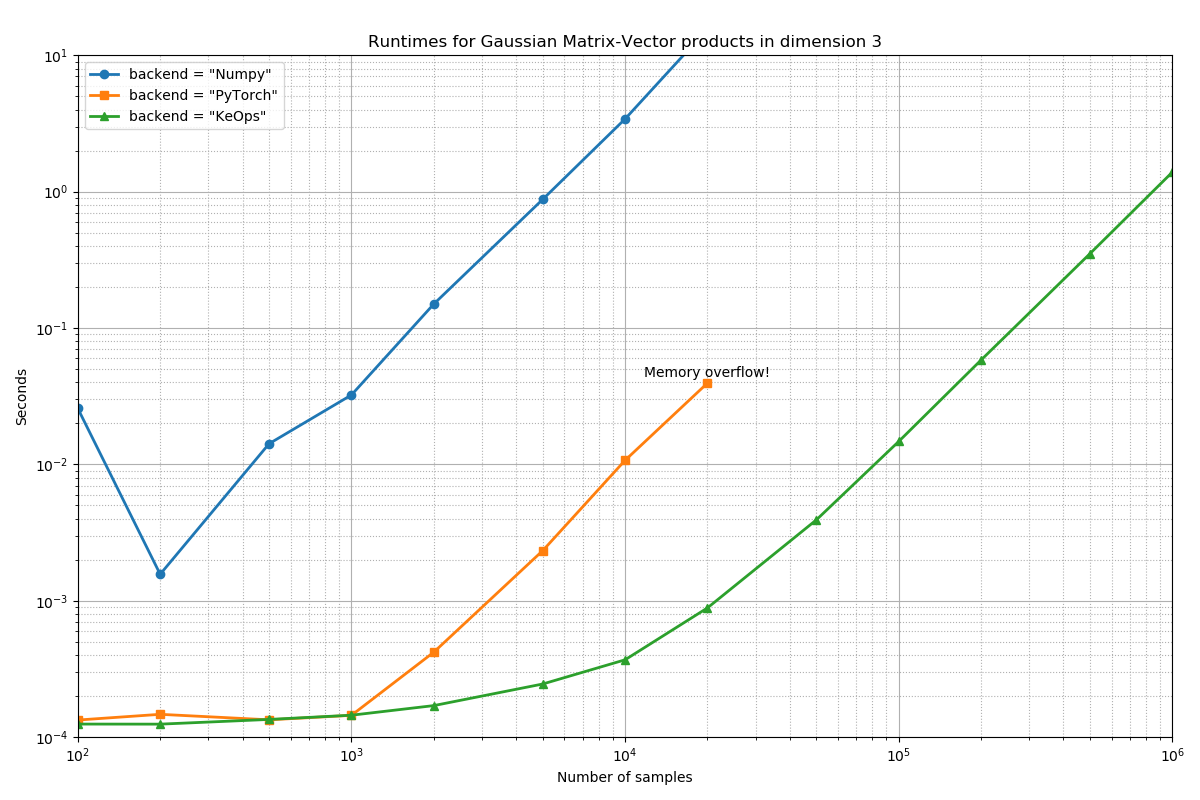
\includegraphics[width=\linewidth]{./images/benchmark.png}
\end{figure}
\end{onlyenv}
\end{frame}

\begin{frame}{R specific benchmarks}

\begin{onlyenv}<1>
Runtime comparison between 
\begin{itemize}
\setitsep{1em}
\item standard \texttt{R}
\item \texttt{RKeOps}
\item \texttt{PyKeOps}
\item \texttt{PyTorch}
\end{itemize}
\end{onlyenv}

\begin{onlyenv}<2>
Different tasks

\begin{itemize}
\small
\setitsep{1em}
\item Matrix-vector product with Gaussian kernel
\item Solving Gaussian kernel linear system
\item 10-iterations of $K$-means algorithm
\item Exact $K$-nearest neighbor search
\end{itemize}
\end{onlyenv}

\begin{onlyenv}<3>
\begin{itemize}
\setitsep{1em}
\item $RKeOps$ outperforms standard $R$ and $PyTorch$ with very large data sizes\\
{\footnotesize (except for $K$-means algorithm because of bad implementation)}
\item Memory overflow with PyTorch on large sample
\item \mybf{RKeOps} able to process data \mybf{larger than GPU memory}
\end{itemize}

\end{onlyenv}

\begin{onlyenv}<4>
\begin{figure}
\centering
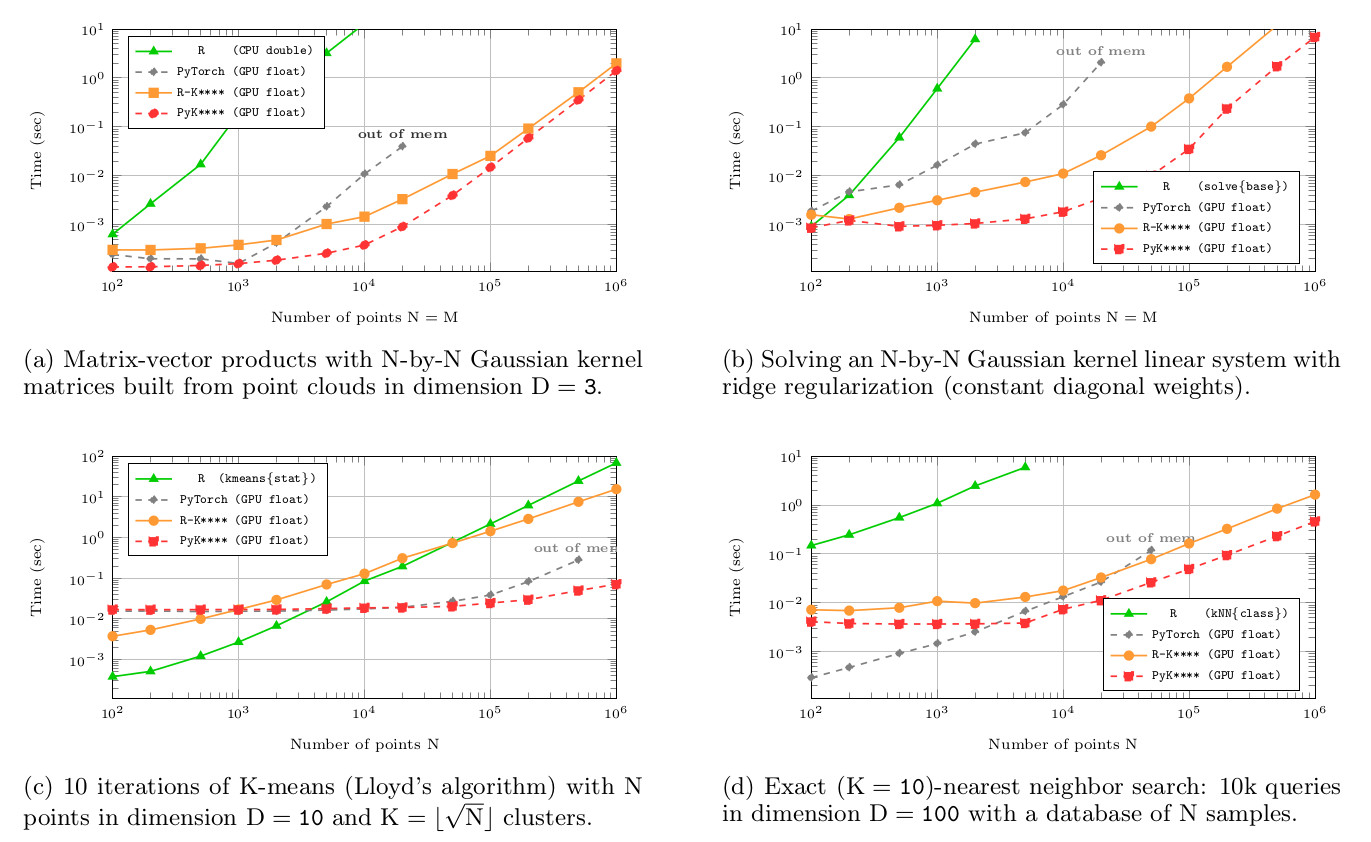
\includegraphics[width=\linewidth]{./images/benchmark2.jpg}
\end{figure}
\end{onlyenv}
\end{frame}


%%%%%%%%%%%%%%%%%%%%%%%%%%%%%%%%%%%%%%%%%%%%%%%%%%%%%%%%%%%%%%%
\section{Implementation}
%%%%%%%%%%%%%%%%%%%%%%%%%%%%%%%%%%%%%%%%%%%%%%%%%%%%%%%%%%%%%%%

%%%%%%%%%%%%%%%%%%%%%%%%
\begin{frame}{Coding generic formulas with KeOps}

\btVFill

\hypertarget{implementation}{}

\mybf{Mathematical formula} with two vectors $\mb x,\mb y\in\RR^D$:
\[
(\mb x, \mb y) \mapsto \exp\big(\langle \mb x, \mb y\rangle\big)
\]

\begin{center}
\small
$\rw$ what I want to compute
\end{center}\bigskip

A formula $F$ in KeOps is first \mybf{encoded as a string} using combinations of elementary operations
\begin{center}
\texttt{"Exp(Scalprod(x,y))"}
\end{center}

\begin{center}
\small
$\rw$ what I have to write
\end{center}

\end{frame}


%%%%%%%%%%%%%%%%%%%%%%%%
\begin{frame}{Under the hood}

The formula $F$ is expanded internally in the C++ code \mybf{using templates}:
\begin{center}
\texttt{F=Exp<Scalprod<X,Y>{}>}
\end{center}
\bigskip

A formula is an instantiation of a variadic recursively defined templated class\medskip

\begin{itemize}
\item[$\rw$] KeOps compiles your operator on the fly to \mybf{compute on GPU}
\end{itemize}

\end{frame}


%%%%%%%%%%%%%%%%%%%%%%%%%%%%%
\begin{frame}{Combining elementary operations}

KeOps proposes a wide range of elementary operations\bigskip

\only<1>{
\begin{itemize}
\setitsep{1em}
\item \mybf{Simple vector operations:} {\small scalar product, norm, distance, normalization, vector/vector element-wise operation (\texttt{+},\texttt{-},\texttt{*},\texttt{/}), etc.}
\item \mybf{Elementary $\RR\to\RR$ functions:} {\small exp, log, inverse, abs, pow, sqrt, sin, cos, etc.}
\end{itemize}
}

\only<2>{
\begin{itemize}
\setitsep{2em}
\item \mybf{Simple matrix operations:} {\small matrix product, etc.}
\item \mybf{Matrix reduction:} {\small sum, min, max, argmin, argmax, etc.}
\end{itemize}
}

\only<3>{
\small

\bigskip\bigskip\bigskip
$\rw$ a formula = \mybf{a combination of these operations}
}

\btVFill
\end{frame}



%%%%%%%%%%%%%%%%%%%%%%%%%%%%%%%%%%%%%%%%%%%%%%%%%%%%%%%%%%%%%%%
\section{Using KeOps}
%%%%%%%%%%%%%%%%%%%%%%%%%%%%%%%%%%%%%%%%%%%%%%%%%%%%%%%%%%%%%%%

\begin{frame}{\url{http://www.kernel-operations.io/}}

\begin{itemize}
\setitsep{2em}
\item Complete documentation
\item Installation instructions (available on CRAN)\medskip
\begin{center}
\texttt{install.packages("rkeops")}
\end{center}

\item Examples
\end{itemize}

\end{frame}


%%%%%%%%%%%%%%%%%%%%%%%%%%%%%
\begin{frame}{KeOps stack}

\begin{onlyenv}<1>
\begin{center}
\url{https://github.com/getkeops/keops}\bigskip

Open source (MIT licence)
\end{center}
\end{onlyenv}

%\begin{onlyenv}<2>
%Dependencies:
%\begin{itemize}
%\setitsep{1em}
%\item \texttt{Cmake} ($\geq$3.10)
%\item \texttt{C++} compiler (g++ $\geq$ 7 or clang) for CPU computing
%\item \texttt{CUDA} compiler (nvcc $\geq$10) and libs \mybf{for GPU computing}
%\end{itemize}
%
%\end{onlyenv}
\end{frame}


%%%%%%%%%%%%%%%%%%%%%%%%%%%%
%\begin{frame}{KeOps user interface}
%
%\begin{itemize}
%\setitsep{2em}
%\item PyKeOps: \texttt{Python} (\texttt{numpy} and \texttt{pytorch})
%\item KeOpsLab: \texttt{Matlab}
%\item \mybf{RKeOps}: \texttt{R}
%\item \texttt{C++} API
%\end{itemize}
%
%\end{frame}



%%%%%%%%%%%%%%%%%%%%%%%%%%%%%%%%%%%%%
\begin{frame}[fragile]{Example in R: single Gaussian convolution}

\begin{onlyenv}<1>
We want to compute\medskip

\[
\myexample{\mbg\gamma_i} = \sum_{\alert{j=1}}^{\alert{N}}  \exp\Big(-s \Vertt \myexample{\mb x_i} - \alert{\mb y_j}\Vertt_2^{\,2}\Big)\,\alert{\mb b_j}
\]
\bigskip

\begin{itemize}
\item[with] $s\in\RR$,\\ $[\mb x_i]_{\myexample{i=1,\hdots,M}} \in\RR^{\myexample{M}\times 3}$, $[\mb y_j]_{\alert{j=1,\hdots,N}} \in\RR^{\alert{N}\times 3}$\\\ and $[\mb b_j]_{\alert{j=1,\hdots,N}} \in\RR^{\alert{N}\times 6}$
\end{itemize}
\end{onlyenv}

\begin{onlyenv}<2>
Compilation on the fly of the operator
\begin{minted}[bgcolor=blue!4,fontsize=\scriptsize,mathescape,tabsize=4]{r}
library(rkeops)

# implementation of a convolution with a Gaussian kernel
formula = "Sum_Reduction(Exp(-s * SqNorm2(x - y)) * b, 0)"

# definition of input arguments
args = c("x = Vi(3)",      # vector indexed by i (of dim 3)
         "y = Vj(3)",      # vector indexed by j (of dim 3)
         "b = Vj(6)",      # vector indexed by j (of dim 6)
         "s = Pm(1)")      # parameter (scalar)
         
# compilation
op <- keops_kernel(formula, args)
\end{minted}
\end{onlyenv}

\begin{onlyenv}<3>
Some data
\begin{minted}[bgcolor=blue!4,fontsize=\footnotesize,mathescape,tabsize=4]{r}
# data and parameter values
nx <- 100
ny <- 150
X <- matrix(runif(nx*3), nrow=nx)   # matrix 100 x 3
Y <- matrix(runif(ny*3), nrow=ny)   # matrix 150 x 3
B <- matrix(runif(ny*6), nrow=ny)   # matrix 150 x 6
s <- 0.2
\end{minted}
\end{onlyenv}

\begin{onlyenv}<4>
Run computations
\begin{minted}[bgcolor=blue!4,fontsize=\footnotesize,mathescape,tabsize=4]{r}
# run computations on GPU (optional)
use_gpu()


# computation
# (order of input list similar to `args`)
res <- op(list(X, Y, B, s))
\end{minted}
\end{onlyenv}

\begin{onlyenv}<5>
Gradient
\begin{minted}[bgcolor=blue!4,fontsize=\footnotesize,mathescape,tabsize=4]{r}
# compile gradient regarding 'x' variable
grad_op <- keops_grad(op, var="x")
\end{minted}
\end{onlyenv}

\end{frame}

%%%%%%%%%%%%%%%%%%%%%%%%%%%%%%%%%%%%%%%%%%%%%%%%%%%%%%%%%%%%%%%
\section{Conclusion}
%%%%%%%%%%%%%%%%%%%%%%%%%%%%%%%%%%%%%%%%%%%%%%%%%%%%%%%%%%%%%%%


%%%%%%%%%%%%%%%%%%%%%%%%%%%%%%%%%%%%%
\begin{frame}{Take-home message: KeOps}
\small
Seamless Kernel Operations...\medskip

\hspace{0.5cm} $\rw$ \myexample{write formulas with simple matrix operations in R}\medskip

...on GPU...\medskip

\hspace{0.5cm} $\rw$ \myexample{fast computations}\medskip

...with auto-differentiation...\medskip

\hspace{0.5cm} $\rw$ \myexample{automatic gradient computation}\medskip

...and without memory overflows\medskip

\hspace{0.5cm} $\rw$ \myexample{tiling implementation}
\end{frame}

%%%%%%%%%%%%%%%%%%%%%%%%%%%%%%%%%%%%%
\begin{frame}[fragile]{In the future?}

\mybf{Lazy evaluation in \texttt{R}} {\small (example below with PyKeOps)}

\begin{minted}[bgcolor=blue!4,fontsize=\footnotesize,mathescape,tabsize=4]{python}
# Symbolic representation of data
x_i = LazyTensor( x[:,None,:] )  # shape (1e6, 1, 3)
y_j = LazyTensor( y[None,:,:] )  # shape ( 1, 2e6,3)

# Symbolic (1e6,2e6,1) matrix of squared distances
D_ij = ((x_i - y_j)**2).sum(dim=2)

# Symbolic (1e6,2e6,1) Gaussian kernel matrix
K_ij = (- D_ij).exp()

## Result (computations on GPU are done here)
a_i = K_ij.sum(dim=1)  # shape (1e6, 1)
\end{minted}

\end{frame}


%%%%%%%%%%%%%%%%%%%%%%%%%%%%%%%%%%%%
\begin{frame}[standout]{}

Thank you for you attention\bigskip\bigskip\bigskip

{\small

\url{https://arxiv.org/abs/2004.11127}\\
(pending publication)\bigskip 

\url{http://www.kernel-operations.io/}\bigskip

\url{https://github.com/getkeops/keops}

}

\end{frame}


\end{document}
